\section{Notation and Terminology}
\label{sec:prelims}

% Initially taken from Kyle's dissertation.

% Temporary definition to allow compilation of lazily copied prelim section:


We begin by recalling several useful definitions related to surface-embedded graphs.  For further background, we refer the reader to Gross and Tucker \cite{gt-tgt-01} or Mohar and Thomassen~\cite{mt-gs-01} for topological graph theory, and to Hatcher~\cite{h-at-02} or Stillwell~\cite{s-ctcgt-93} for surface topology and homology.


\subsection{Surfaces and Curves}

A \EMPH{surface} (more formally, a \emph{2-manifold with boundary}) is a compact Hausdorff space in which every point has an open neighborhood homeomorphic to either the plane $\Real^2$ or a closed halfplane $\set{(x,y)\in \Real^2\mid x\ge 0}$.  The points with halfplane neighborhoods make up the \EMPH{boundary} of the surface; every component of the boundary is homeomorphic to a circle.
A surface is \EMPH{non-orientable} if it contains a subset homeomorphic to
the M\"obius band, and \EMPH{orientable} otherwise. In this dissertation, we consider only compact, connected, and orientable surfaces.

A \EMPH{path} in a surface $\Sigma$ is a continuous function $p\colon [0,1]\to\Sigma$.
A \EMPH{loop} is a path whose endpoints~$p(0)$ and~$p(1)$ coincide;
we refer to this common endpoint as the \EMPH{basepoint} of the loop.
An \EMPH{arc} is a path internally disjoint from the boundary of~$\Sigma$
whose endpoints lie on the boundary of $\Sigma$.
A \EMPH{cycle} is a continuous function $\gamma\colon S^1\to\Sigma$;
the only difference between a cycle and a loop is that a loop has a
distinguished basepoint.
We say a loop~$\ell$ and a cycle~$\gamma$ are \EMPH{equivalent} if, for some
real number~$\delta$, we have~$\ell(t) = \gamma(t + \delta)$ for
all~$t \in [0,1]$.
We collectively refer to paths, loops, arcs, and cycles as \EMPH{curves}.
A curve is \EMPH{simple} if it is injective; we usually do not distinguish between simple curves and their images in $\Sigma$.
A simple curve~$p$ is \EMPH{separating} if~$\Sigma \setminus p$ is disconnected.

The \EMPH{reversal}~$\rev(p)$ of a path~$p$ is defined by
setting~$\rev(p)(t) = p(1-t)$. The \EMPH{concatenation}~$p \cdot q$ of two
paths~$p$ and~$q$ with~$p(1)=q(0)$ is the path created by
setting~$(p\cdot q)(t) = p(2t)$ for all~$t \leq 1/2$
and~$(p\cdot q)(t) = q(2t-1)$ for all~$t \geq 1/2$. Finally, let~$p[x,y]$
denote the subpath of a path~$p$ from point~$x$ to point~$y$.

The \EMPH{genus} of a surface $\Sigma$ is the maximum number of disjoint simple cycles in $\Sigma$ whose complement is connected.
 Up to homeomorphism,
there is exactly one orientable surface and one non-orientable surface with any genus $g\ge 0$ and any number of
boundary cycles $b\ge 0$.
Orientable surfaces with~$b$ boundary components are differentiated by their \EMPH{Euler characteristic} ${\chi = 2 - 2g - b}$ (for non-orientable surfaces, ${\chi = 2 - g - b}$).


\subsection{Graph Embeddings}

An \EMPH{embedding} of an undirected graph $G=(V,E)$ on a surface $\Sigma$ maps vertices to distinct points and edges to simple, interior-disjoint paths.  The \EMPH{faces} of the embedding are maximal connected subsets of $\Sigma$ that are disjoint from the image of the graph.
We may denote an edge~$uv \in E$ as~$f | g$ if it is incident to faces~$f$ and~$g$.
An embedding is \EMPH{cellular} if each of its faces is homeomorphic to the plane; in particular, in any cellular embedding, each component of the boundary of $\Sigma$ must be covered by a cycle of edges in $G$.  Euler's formula implies that any cellularly embedded graph with $n$ vertices, $m$ edges, and $f$ faces lies on a surface with Euler characteristic $\chi = n-m+f$, which implies that $m = O(n+g)$ and $f=O(n+g)$
if the graph is simple.
We consider only such
cellular embeddings of genus $g=O(n^{1-\eps})$, so that the overall complexity of the embedding is $O(n)$.

Any cellular embedding on an orientable surface can be encoded combinatorially
by a \EMPH{rotation system}, which records the counterclockwise order of edges
incident to each vertex.
Two paths or cycles in a combinatorial surface \EMPH{cross} if no continuous infinitesimal perturbation makes them disjoint; if such a perturbation exists, then the paths are \EMPH{non-crossing}.

We redundantly use the term \EMPH{arc} to refer to a walk in the graph whose endpoints are boundary vertices.  Likewise, we use the term \EMPH{cycle} to refer to a closed walk in the graph. 
Note that cycles may contain the same vertex or edge more than once.

\begin{figure}[t]
\centering
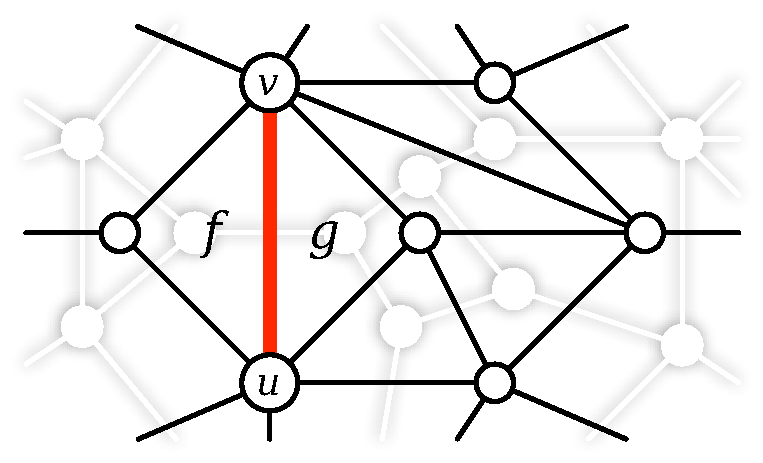
\includegraphics[height=0.9in]{Fig/primal}\quad
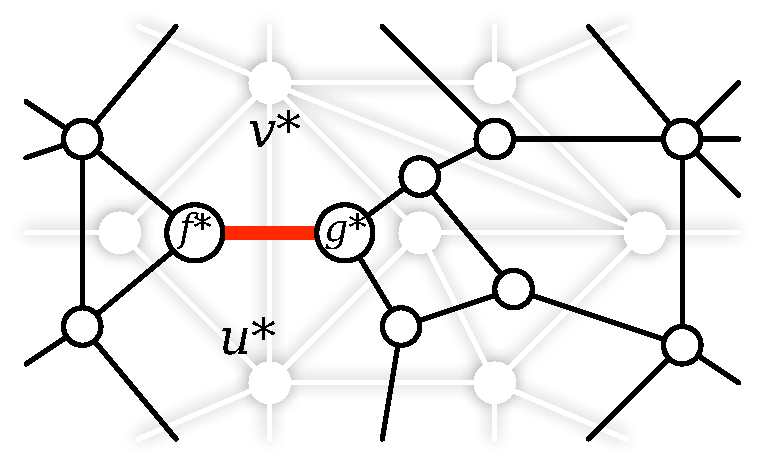
\includegraphics[height=0.9in]{Fig/dual}
\caption{Graph duality.  One edge $uv$ and its dual $(uv)^* =
f^*g^*$ are emphasized.} \label{fig:prelims_primaldual}
\end{figure}

Any undirected graph~$G$ embedded on a surface~$\Sigma$ without boundary has a
\EMPH{dual graph}~$G^*$, which has a vertex~$f^*$ for each face~$f$ of~$G$,
and an edge~$e^*$ for each edge~$e$ in~$G$ joining the vertices dual to the
faces of~$G$ that~$e$ separates. The dual graph~$G^*$ has a natural cellular
embedding in~$\Sigma$, whose faces corresponds to the vertices of~$G$.
See Figure~\ref{fig:prelims_primaldual}.
For any subgraph~${F = (U, D)}$ of~$G=(V,E)$, we write~$G \setminus F$
to denote the edge-complement~$(V,E \setminus D)$. We also abuse notation
by writing~$F^*$ to denote the subgraph of~$G^*$ corresponding to any
subgraph~$F$ of~$G$.
Further, we may sometimes use~$D$ to refer to an edge set or the subgraph~$F = (V, D)$,
but it should be clear which we mean from context.

A \EMPH{tree-cotree decomposition}~$(T,L,C)$ of an undirected
graph~$G$ embedded on a surface without boundary 
is a partition of the edges into three disjoint subsets;
a spanning tree~$T$ of~$G$, a spanning cotree~$C$ (the dual of a spanning
tree~$C^*$ of~$G^*$), and leftover edges~$L=G \setminus (T \cup C)$.
Euler's formula implies that in any tree-cotree decomposition, the set~$L$
contains exactly~$2g$ edges~\cite{e-dgteg-03}.
The definitions for dual
graphs and tree-cotree decompositions given above
extend to surfaces with boundary, but
we do not require these extensions in this dissertation.

For some of the problems we consider in Chapters~\ref{chap:non-trivial} and~\ref{chap:max-flow}, the input is actually a \emph{directed} edge-weighted (or capacitated)
graph~$G$ with a cellular embedding on some surface.
We use the
notation~$u \arcto v$ to denote the directed \EMPH{dart} from vertex~$u$ to vertex~$v$, and let~$\vec{E}$ be the set of darts in~$G$.
Without loss of generality, we consider only \EMPH{symmetric} directed graphs,
in which the reversal~$v \arcto u$ of any dart~$u \arcto v$ is another dart,
possibly with infinite weight (or~$0$ capacity).
We also assume that in the cellular embedding,
the images of any edge in~$G$ and its reversal coincide (but with opposite
orientations).
The two darts~$u \arcto v$ and~$v \arcto u$ therefore define an \EMPH{edge}~$uv$
with a canonical orientation~$u \arcto v$; edge~$vu$ does not necessarily exist even though~$uv$ does.
Thus, like Cabello \etal~\cite{ccl-fsncd-10} and Erickson~\cite{e-sncds-11},
we implicitly model directed graphs as \emph{undirected graphs with asymmetric
edge weights}.
We may denote dart~$u \arcto v$ as~$f \uparrow g$ if faces~$f$ and~$g$ lie to its left and right respectively.
The dual of any dart~$f \uparrow g$ is~$f^* \arcto g^*$.
Note that the duality of darts is \emph{not} an involution the way we have specified the orientation of the dual dart here.

Let~$p = v_0 \arcto v_1 \arcto \dots \arcto v_k$ be a simple directed cycle
or arc in an
embedded graph~$G$. We say an edge~$u \arcto v_i$ \EMPH{enters~$p$
from the left}
(resp. right) if the vertices~$v_{i-1}$,~$u$, and~$v_{i+1}$ (module~$k$
in the case of a cycle) are ordered
clockwise (resp. counterclockwise) around~$v_i$, according to the
embedding's rotation system. An edge~$v_i \arcto u$ \EMPH{leaves~$p$ from the
left} (resp. right) if its reversal~$u \arcto v_i$ enters~$p$ from the
left (resp. right).
If~$p$ is an arc,
the above definitions require that~$0 < i < k$ and that~$u$
is not a vertex in~$p$. Recall an arc's endpoints lie on boundary cycles.
Let~$t_0 v_0$ and~$v_0 w_0$ be the boundary edges
incident to~$v_0$ with vertices~$t_0$, $v_1$, and $w_0$ appearing in clockwise
order around~$v_0$. We say~$t_0 \arcto v_0$ enters~$p$ from the left.
We say~$w_0 \arcto v_0$ enters~$p$
from the right. Similarly,
if~$t_k v_k$ and~$v_k w_k$ are boundary edges incident to~$v_k$ with
vertices~$t_k$, $w_k$, and~$v_{k-1}$ appearing in clockwise order around~$v_k$,
we say~$t_k \arcto v_k$ enters~$p$ from the left and~$w_k \arcto v_k$
enters~$p$ from the right. Finally, we treat~$t_0$ as~$v_{-1}$ and~$t_k$
as~$v_{k+1}$ to define entering from the left (resp. right) for any
other edges~$u \arcto v_0$ or~$u \arcto v_k$ where~$u$ does not appear in~$p$.

\subsection{Homotopy and Homology}

Two paths~$p$ and~$q$ in $\Sigma$ are \EMPH{homotopic} if one can be
continuously deformed into the other without changing their endpoints.
More formally, a \EMPH{homotopy} between~$p$ and~$q$ is a
continuous map $h\colon {[0,1]\times [0,1] \to \Sigma}$ such that $h(0,\cdot) = p$, $h(1,\cdot) = q$, $h(\cdot, 0)=p(0)=q(0)$, and $h(\cdot,1)=p(1)=q(1)$.
Homotopy defines an equivalence relation over the set of paths with any
fixed pair of endpoints. The set of homotopy classes of loops in~$\Sigma$
with basepoint~$x_0$ defines a group~$\pi_i(\Sigma,x_0)$ under concatenation,
called the \EMPH{fundamental group} of~$\Sigma$. (For all basepoints~$x_0$
and~$x_1$, the groups~$\pi_i(\Sigma,x_0)$ and~$\pi_i(\Sigma,x_1)$ are
isomorphic.) A cycle is \EMPH{contractible} if it is homotopic to a constant
map.
Given a weight function on the darts of~$G$, we say a directed path or cycle is \EMPH{tight} if it has minimum total weight (counting edges with multiplicity) for its homotopy class.

Homology is a coarser equivalence relation than homotopy, with nicer
algebraic properties.  Like several earlier papers \cite{cf-qhc2-07,
cf-qhc-08, dls-chtl-07, dlsc-cgaht-08}, we will consider only
one-dimensional cellular homology with coefficients in the finite
field $\Z_2$; this restriction allows us to radically simplify our
definitions.  For a more general treatment of homology, we refer the
reader to our companion paper~\cite{cen-hfcc-09} or to standard
references on topology \cite{h-at-01, s-ctcgt-93, z-tc-05}.

%\note{Reviewer 2 suggests: "you should probably emphasize that the even and boundary subgraphs are vector spaces over $Z_2$, and define $\oplus$."}

Fix a cellular embedding of an undirected graph $G$ on a surface with genus $g$ and $b$ boundaries.  An \EMPH{even subgraph} is a subgraph of $G$ in which every node has even degree, or equivalently, the union of edge-disjoint cycles.  A \EMPH{boundary subgraph} is the boundary of the union of a subset of faces of $G$; for example, every separating cycle is a boundary subgraph.
%For planar graphs, every even subgraph is a boundary subgraph, but this equivalence does not extend to higher-genus embeddings.
Two even subgraphs are \EMPH{homologous}, or in the same \EMPH{homology class}, if their symmetric difference is a boundary subgraph.
%Equivalently, two even subgraphs are homologous if one can be continuously deformed into the other via a deformation that may include splitting cycles at self-intersection points, merging intersecting pairs of cycles, or adding or deleting contractible cycles.
Boundary subgraphs are also called \EMPH{null-homologous}.  Any two homotopic cycles are homologous, but homologous cycles are not necessarily homotopic; see Figure \ref{F:homology}.  Moreover, the homology class of a cycle can contain even subgraphs that are not cycles; see Figure \ref{F:homology2}.

%\note{Reviewer 2 says: "Figure 1, left, is hard to understand (draw the hidden parts of the curves".  Erin: I disagree!  I wouldn't change it, but that's your call, Jeff.}

%\note{Jeff: Um.  The `hidden' parts of the curves are already there: thinner, lighter, and cased.  I don't know how to make them any clearer!  The lack of visualization ability in the SOCG community never ceases to amaze me.}

\begin{figure}[htb]
\centering
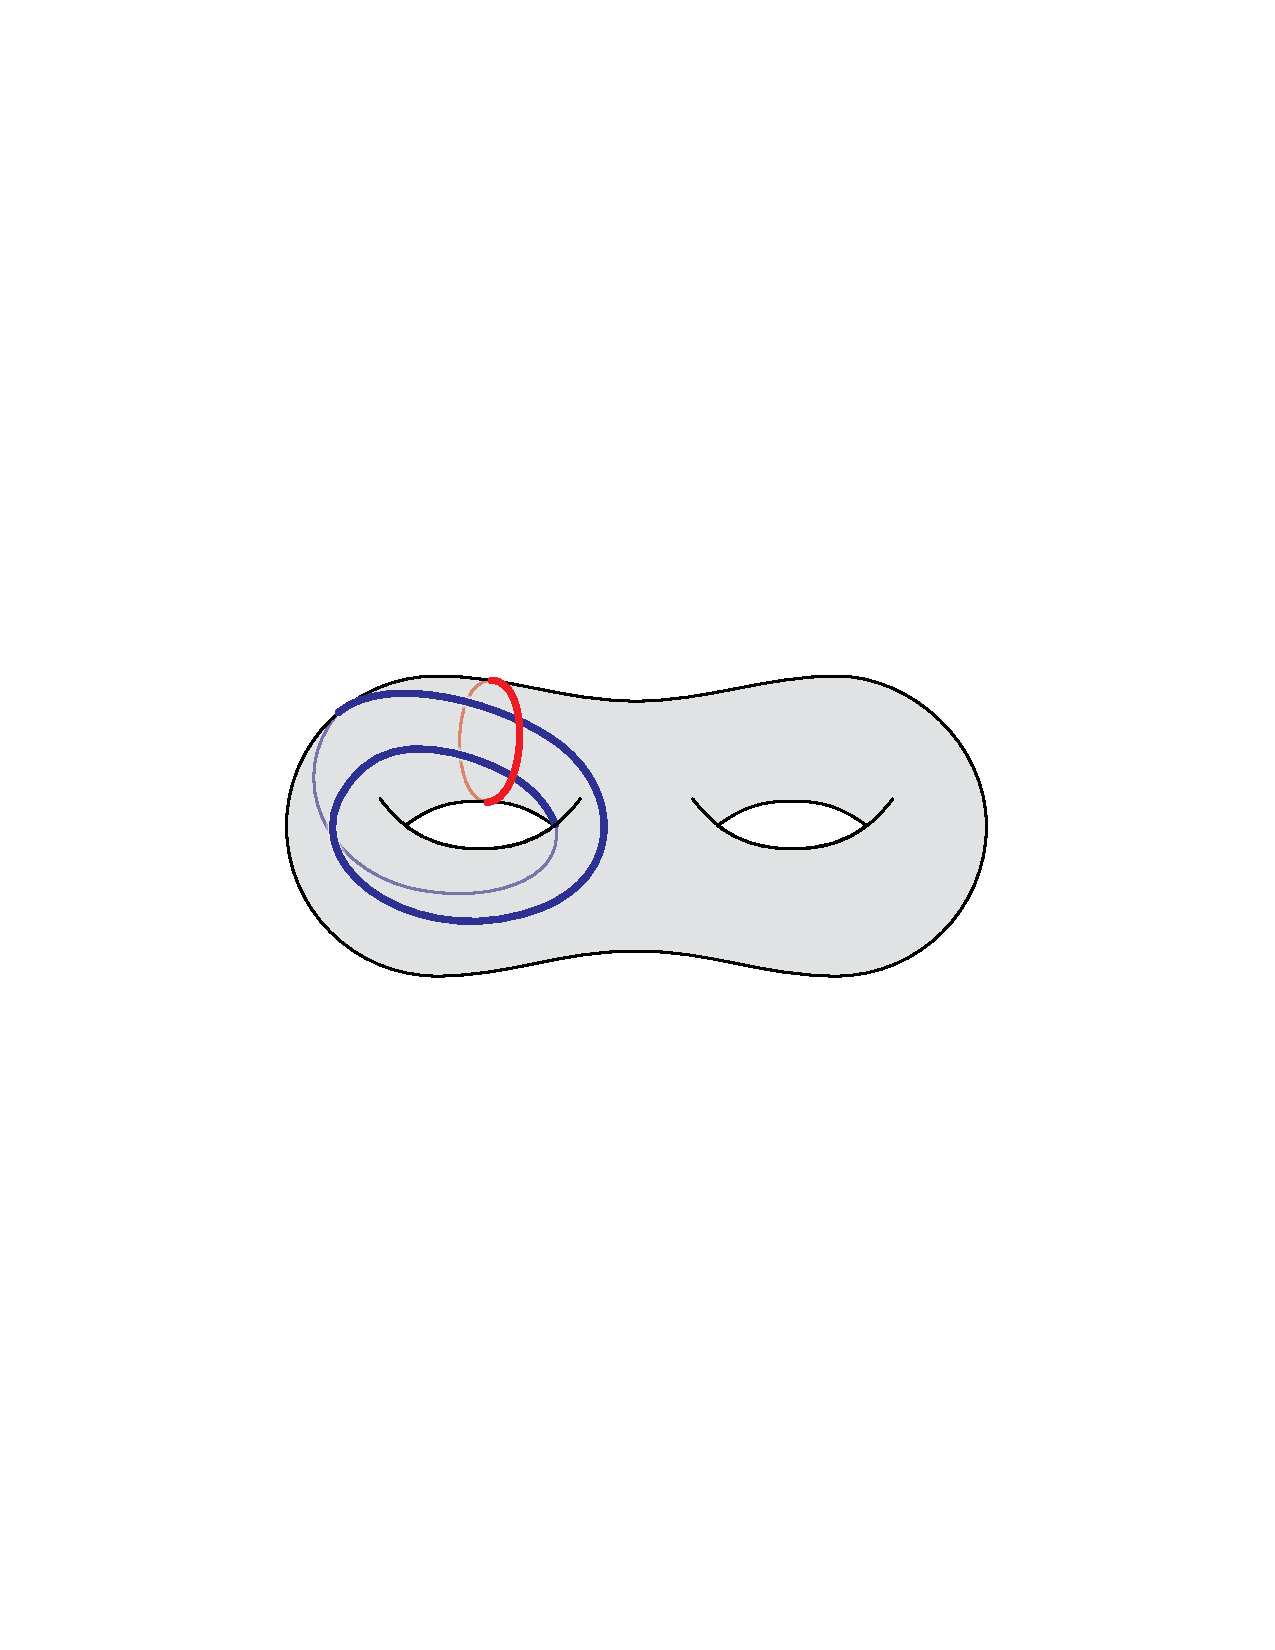
\includegraphics[height=0.75in]{Fig/homologous3}\\[2ex]
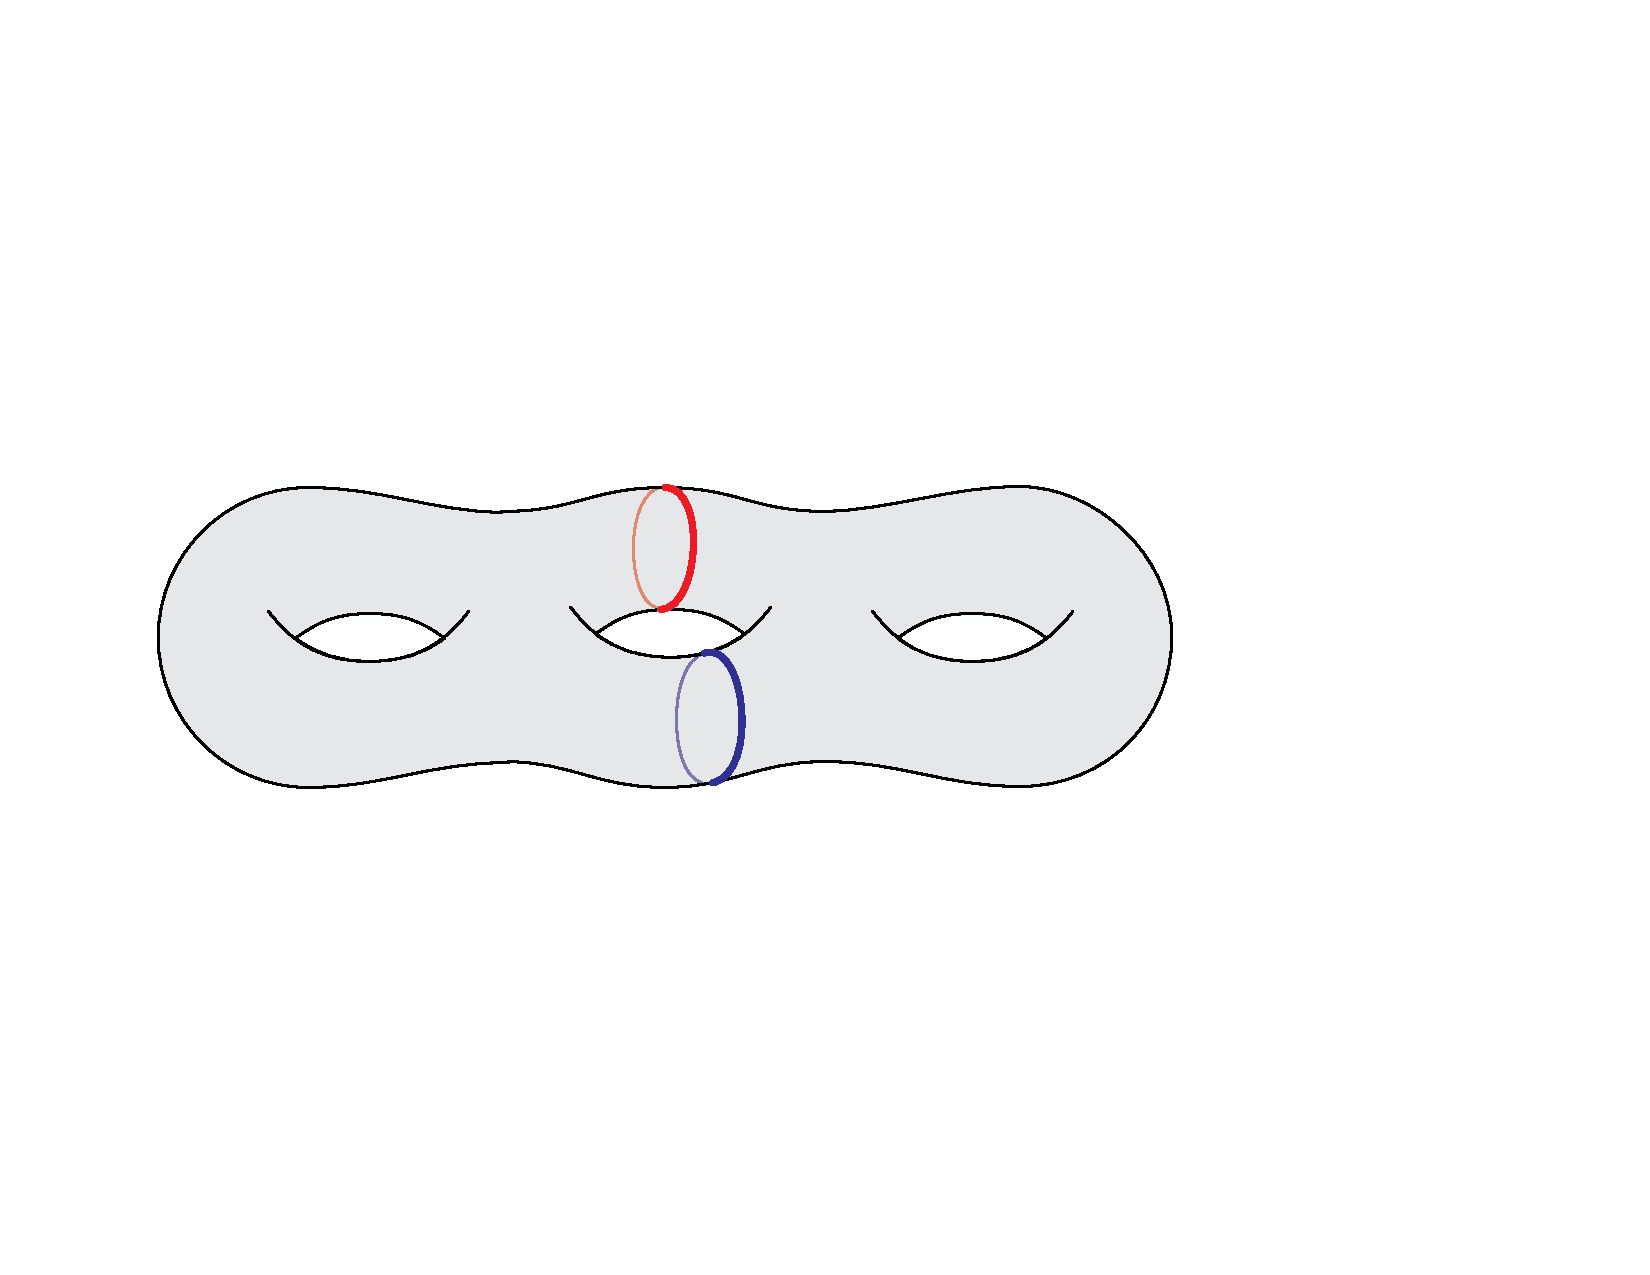
\includegraphics[height=0.75in]{Fig/homologous2}
\caption{Homologous pairs of cycles that are not homotopic.  (Lighter portions of the curves are on the back side of the surface.)}
\label{F:homology}
\end{figure}

\begin{figure}[htb]
\centering
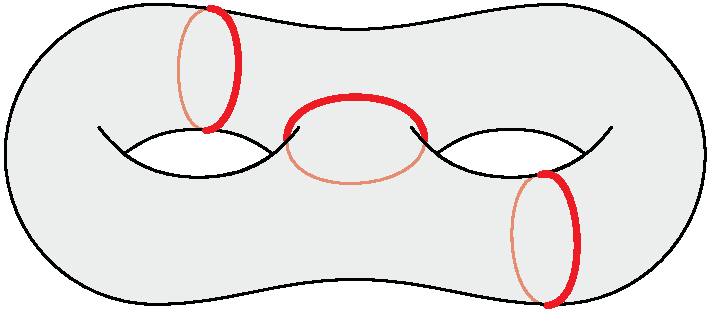
\includegraphics[height=0.75in]{Fig/homologous1}
\caption{Each cycle is homologous to the union of the other two.}
\label{F:homology2}
\end{figure}

\subsection{Flows and Cuts}
Consider again homology with coefficients in~$\R$.
We will often refer to $1$-chains as \EMPH{flows} or \EMPH{coflows} depending on if we are focusing on the primal or dual graph.
Any flow can be decomposed to a set of weighted paths and cycles.
For any capacity function~$c : \vec{E} \to \R$ on the \emph{darts}, we say a flow~$\phi$ is \EMPH{feasible} if $-c(v \arcto u) \leq \phi(uv) \leq c(u \arcto v)$.
Note that capacity functions do not necessarily have to be non-negative for feasibility to be well defined.
Given a coflow~$\theta$ we define the capacity of~$\theta$ with respect to~$c$ as follows.
Let~$c' : E \to \R$ be a function on the edges such that~$c'(uv) = c(u \arcto v)$ if~$\theta(uv) \geq 0$ and~$c'(uv) = -c(v \arcto u)$ if~$\theta(uv) < 0$.
The capacity of~$\theta$ with respect to~$c$ is the dot product~$\langle \theta, c' \rangle$.

For $s,t \in V$, an $s,t$-\EMPH{flow} is a 1-chain $\phi: E \to \R$ such that $\partial \phi(v) = 0$ for all $v \in V\backslash \{s,t\}$.
The value of an $s,t$-flow~$\phi$ is $\sum_{s \arcto v} \phi(s \arcto v)$.
A \EMPH{maximum $s,t$-flow} with respect to a capacity function~$c$ is a feasible flow of highest value.
For a flow $\phi$, the \EMPH{residual capacity} function $c_{\phi}: \vec{E} \to \R$ is defined as $c_{\phi}(u \arcto v) = c(u \arcto v) - \phi(u \arcto v)$.
Given a capacity function~$c$, we may refer to the \EMPH{residual graph $G_{\phi}$} when discussing the graph~$G$ coupled with residual capacity function~$c_\phi$.
The \EMPH{dual residual graph}~$G^*_{\phi}$ is simply the dual graph~$G^*$ coupled with the residual capacity function~$c_\phi$.

An \EMPH{cut} in~$G = (V, E)$ is defined as a subset of vertices~$S \subseteq V$; we refer to $S$ and $T = V\backslash S$ as different \EMPH{sides} of the cut.
Given two vertices~$s$ and~$t$ with $s \in S$ and $t \in T$, we say $S$ is an
\EMPH{$s,t$-cut}.
A dart~$u \arcto v$ (and its associated edge~$uv$ or~$vu$) \EMPH{crosses} a cut $S$ if exactly one of $u$ and $v$ lie in $S$.
In particular, $u \arcto v$ crosses $S$ in the \EMPH{forward} direction if $u\in S$ and in the \EMPH{backward} direction if $v \in S$.
For a cut $S$ we use the notation \EMPH{$\Gamma^+(S)$} to denote the set of all darts that cross $S$ in the \emph{forward} direction.
We define \EMPH{$\Gamma^-(S)$} as the set of darts that cross $S$ in the backward direction.
A walk $W$ crosses a cut $S$ $k$ times if  there are $k$ edges of $W$ that cross $S$.

Given a dart capacity function~$c : \vec{E} \to \R$, the value or capacity of a cut~$S$ is~$\sum_{u \arcto v \in \Gamma^+(S)} c(u \arcto v)$.
Equivalently, the capacity of a cut~$S$ is equal to the capacity of a coflow~$\theta$ such that~$\theta(u \arcto v) = 1$ if~$u \arcto v \in \Gamma^+(S)$ and~$\theta(u \arcto v) = 0$ if~$uv$ does not cross~$S$.
A \EMPH{minimum $s,t$-cut} of~$G$ with respect to capacity function~$c$ is an $s,t$-cut of minimum value.
The well known maximum-flow/minimum-cut theorem of Ford and Fulkerson~\cite{ff-mfn-56} states that for any non-negative capacity function $c$, the value of a maximum feasible $s,t$-flow is equal to the value of a minimum $s,t$-cut.


\subsection{Covering Spaces and Cutting}

A continuous map~$\pi : \Sigma' \to \Sigma$ between two surfaces is called a
\EMPH{covering map} if each point~$x \in \Sigma$ lies in an open
neighborhood~$U$ such that (1)~$\pi^{-1}(U)$ is a countable union of disjoint
open sets~$U_1 \cup U_2 \cup \cdots$ and (2) for each~$i$, the
restriction~$\pi |_{U_i} : U_i \to U$ is a homeomorphism. If there is a covering
map~$\pi$ from~$\Sigma'$ to~$\Sigma$, we call~$\Sigma'$ a \EMPH{covering space}
of~$\Sigma$. The \EMPH{universal cover}~$\tilde{\Sigma}$ is the unique
simply-connected covering space of~$\Sigma$ (up to homeomorphism).
The universal cover is so named because it covers every path-connected
covering space of~$\Sigma$.

For any path~$p : [0,1] \to \Sigma$ such that~$\pi(x') = p(0)$ for some
point~$x' \in \Sigma'$, there is a unique path~$p'$ in~$\Sigma'$, called
a \EMPH{lift} of~$p$, such that~$p'(0) = x'$ and~$\pi \circ p' = p$. We also
say that~$p$ \EMPH{lifts} to~$p'$. Conversely, for any path~$p'$ in~$\Sigma'$,
the path~$\pi \circ p'$ is called a \EMPH{projection} of~$p'$.

We define a lift of a cycle~$\gamma : S^1 \to \Sigma$ to be the infinite
path~$\gamma' : \R \to \Sigma'$ such that
${\pi(\gamma'(t)) = \gamma(t \mod 1)}$
for all real~$t$. We call the path obtained by restricting~$\gamma'$ to any
unit interval a \EMPH{single-period lift} of~$\gamma$; equivalently, a
single-period lift of~$\gamma$ is a lift of any loop equivalent to~$\gamma$.
We informally say that a cycle is the~\EMPH{projection} of any of its
single-period lifts.

\EMPH{Cutting} a combinatorial surface along a cycle or  arc modifies both the surface and the embedded graph.
For any combinatorial surface $S = (\Sigma, G)$ and any simple cycle or arc $\gamma$ in~$G$, we define a new combinatorial surface \EMPH{$S \snip \gamma$} by taking the topological closure of $\Sigma \backslash \gamma$ as the new underlying surface; the new embedded graph contains two copies of each vertex and edge of $\gamma$, each bordering a new boundary.
Similar to covering spaces, we define the~\EMPH{projection} of a curve in~$S \snip \gamma$ as the natural mapping of points (or vertices and edges) to~$S$.
